\documentclass{article}
\usepackage{graphicx}
\usepackage{amsmath}
\usepackage{amsfonts}
\usepackage{bookmark}
\usepackage{booktabs}
\usepackage{exercises}
\graphicspath{ {./images/4.4} }
\usepackage{indentfirst}
\usepackage{amsthm}
\usepackage{yhmath}
\usepackage{placeins}
\newcommand*{\oldneg}{\mathord{\sim}}
\newcommand\showdiv[1]{\overline{\smash{)}#1}}
\newcommand\Mydiv[1]{%
\smash{\raise.3ex\hbox{$\big)$}}\mkern-8mu
        \overline{\enspace\strut#1}}
\setlength{\tabcolsep}{5pt}
\theoremstyle{definition}
\newtheorem{definition}{Definition}

\setlength{\parindent}{.5in}
\setlength{\parskip}{12pt}
\renewcommand{\arraystretch}{2}
\newcommand{\?}{\stackrel{?}{=}}

\title{4.4 Answers}
\begin{document}
\maketitle

\section*{1}
A logarithm with base 10 is called a common logarithm.

\section*{2}
Let $y=5^x$ be the function $f$, and the $y=\log_5 x$ be the function $g$. Then $f(g(x))=f(\log_5 x)=5^{\log_5 x}=x$ and 
$g(f(x))=g(5^x)=\log_5{5^x}=x$, meaning $y=5^x$ and $y=\log_5 x$ are inverse functions.

\section*{3}
\[ 4^2=16 \]

\section*{4}
\[ 7^3=343 \]

\section*{5}
\[ 6^{-2}=\frac{1}{36} \]

\section*{6}
\[ 64^0=1 \]

\section*{7}
Recall that $\log_b x=y$ iff $b^y=x$. In the answer, however, we would have $\log_b x=y$ iff $b^x=y$, which is incorrect. Instead, the answer 
should be \[ \log_2 \frac{1}{8}=-3 \]

\section*{15}
\[ \log_{16}\frac{1}{4}=-\frac{1}{2} \]

\section*{16}
\[ \log_{\frac{1}{4}}16={-2} \]

\section*{17}
\[ \log_{8}512=\log_{2^3}2^9=3 \]

\section*{18}
\[ \log_{5}625=4 \]

\section*{19}
\[ \log_{11}121=2 \]

\section*{26}
\[ \log{0.746}\approx -0.1273 \]

\section*{27}
\[ \ln{110}\approx 4.7 \]

\section*{30}
\[ 30^{\log_{30}4}=4 \]

\section*{31}
\[ 10^{\log{8}}=8 \]

\section*{32}
\[ \log_6{36}^x=\log_6{6^2}^x=\log_6{6^{2x}}=2x \]

\section*{33}
\[ \log_3{81}^x=\log_3{3^4}^x=\log_3{3^{4x}}=4x \]

\section*{35}
\[ \log_2{32}^x=\log_2{2^5}^x=\log_2{2^{5x}}=5x \]

\section*{36}
\[ \log{100^x}=\log{10^{2x}}=2x \]
B

\section*{40}
\[ y=\log_{\frac{1}{2}}x \] \[ x=\log_{\frac{1}{2}}y \] \[ (\frac{1}{2})^x=y \]

\section*{41}
\[ y=e^{x+2} \]
\[ x=e^{y+2} \]
\[ \ln{x}=y+2 \]
\[ \ln{x}-2=y \]

\section*{42}
\[ y=2^x-3 \] \[ x=2^y-3\] \[ x+3=2^y \] \[ \log_2(x+3)=y \]

\section*{43}
\[ y=\ln(x+1) \] \[ x=\ln(y+1) \] \[ y+1=e^{x} \] \[ e^{x}-1=y \]

\section*{44}
\[ y=6+\log{x} \] \[ x=6+\log{y} \] \[ x-6=\log{y} \] \[ 10^{x-6}=y \]

\section*{46}
(In this problem and number 52, there should be an arror pointing downwards on the left side of the graph)\newline
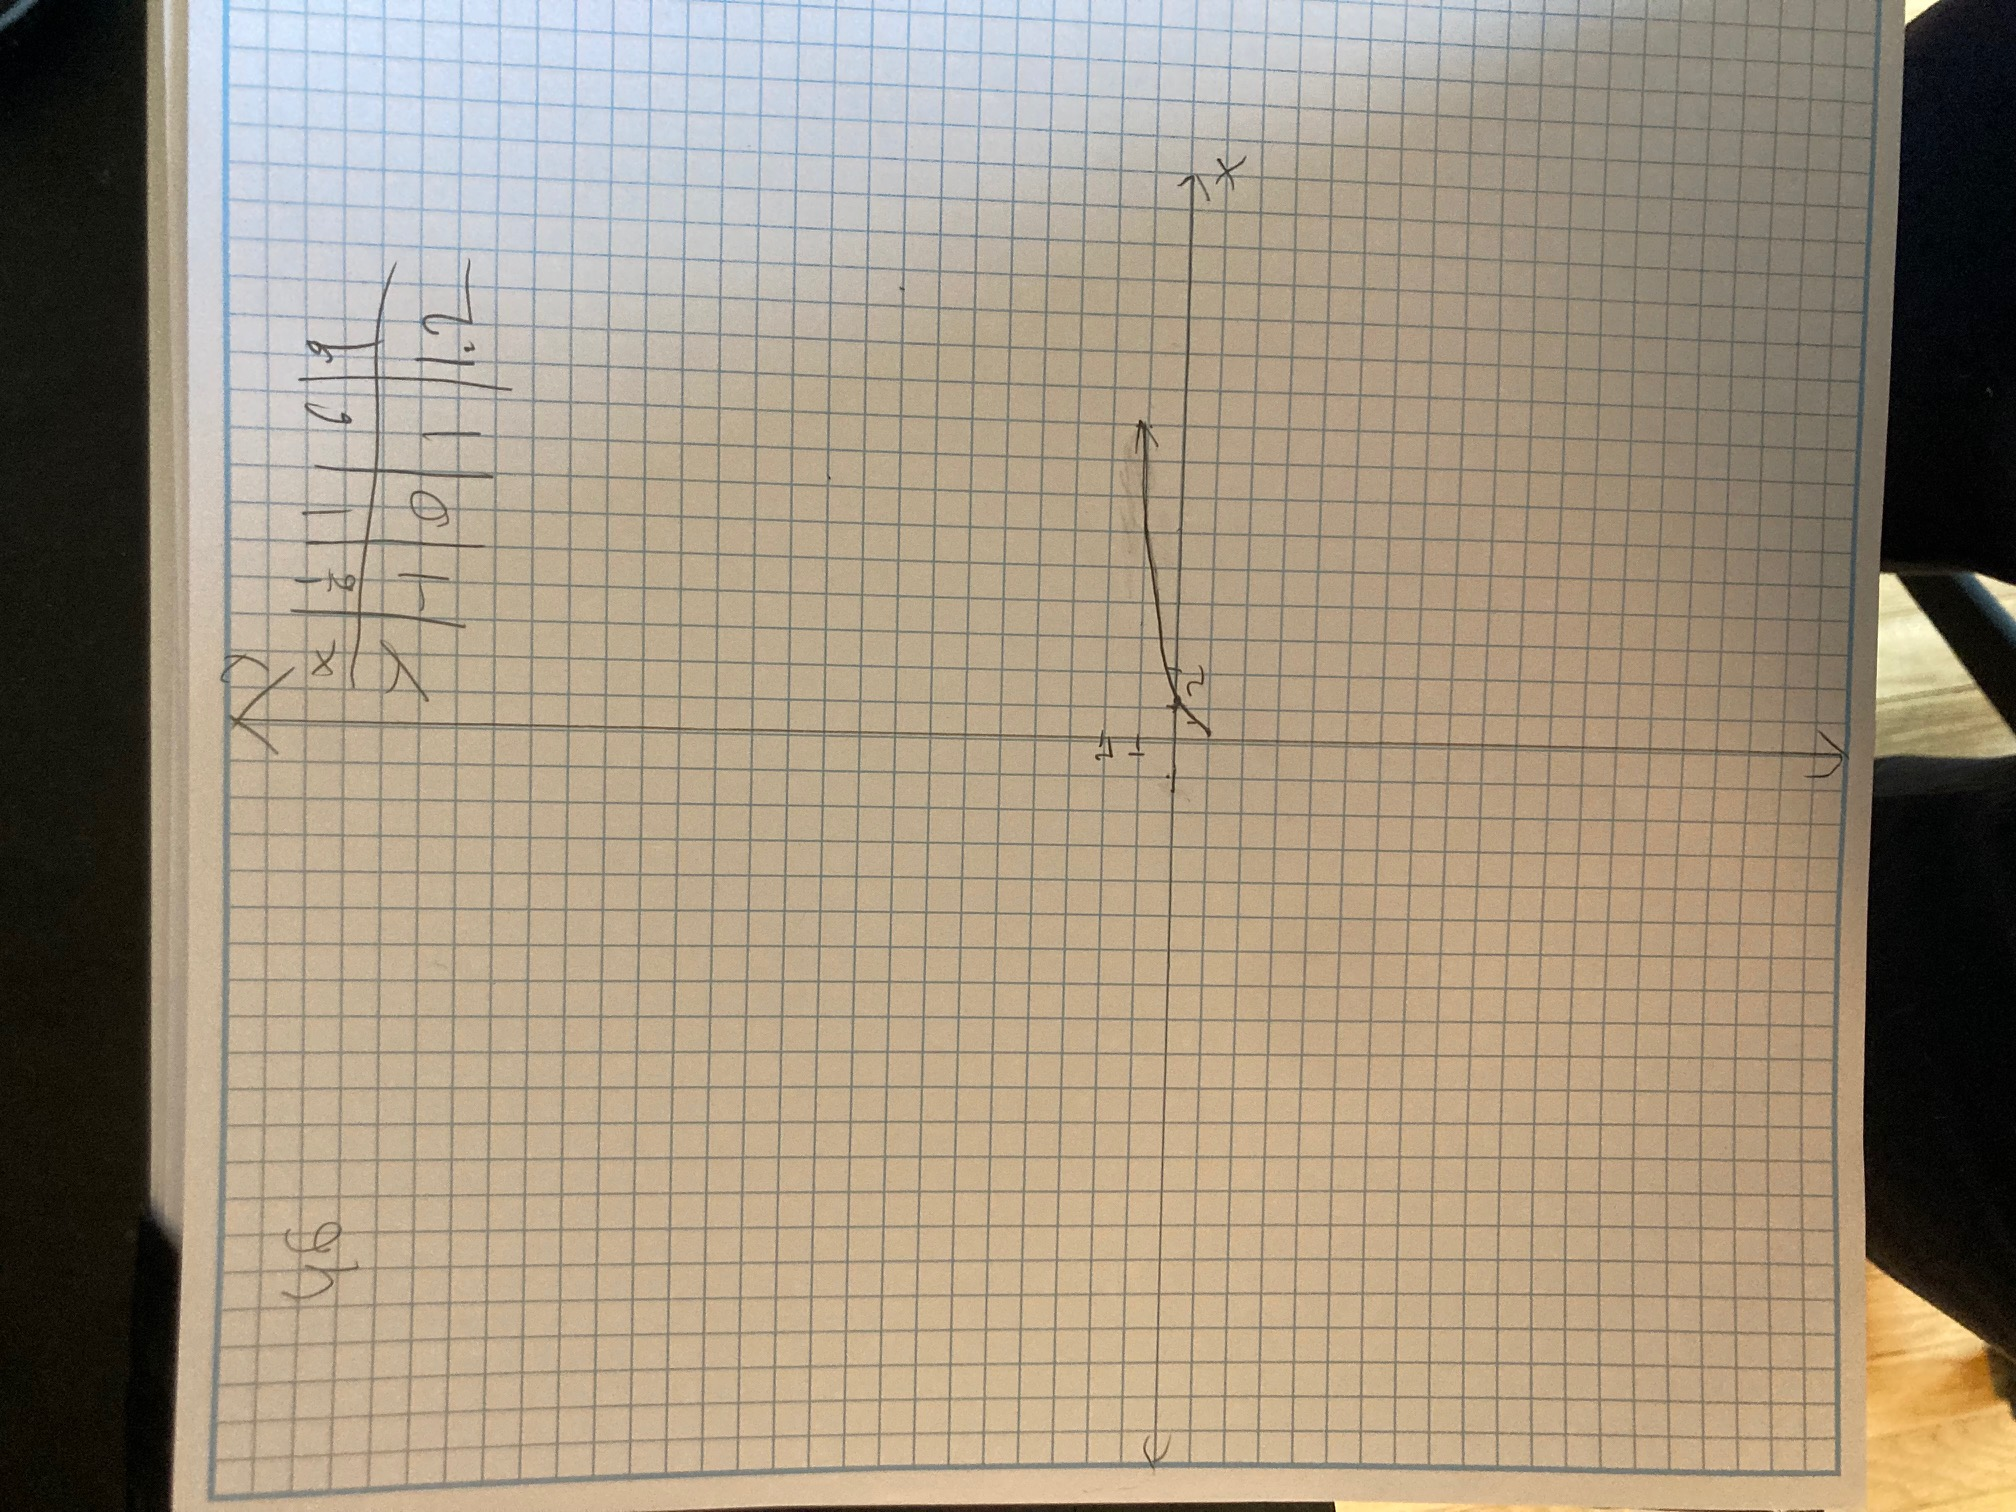
\includegraphics[width = 4in, height = 4in, angle=-90]{46}
\newline The domain of the function is all real numbers $>0$, and the range of the function is all real numbers.

\section*{52}
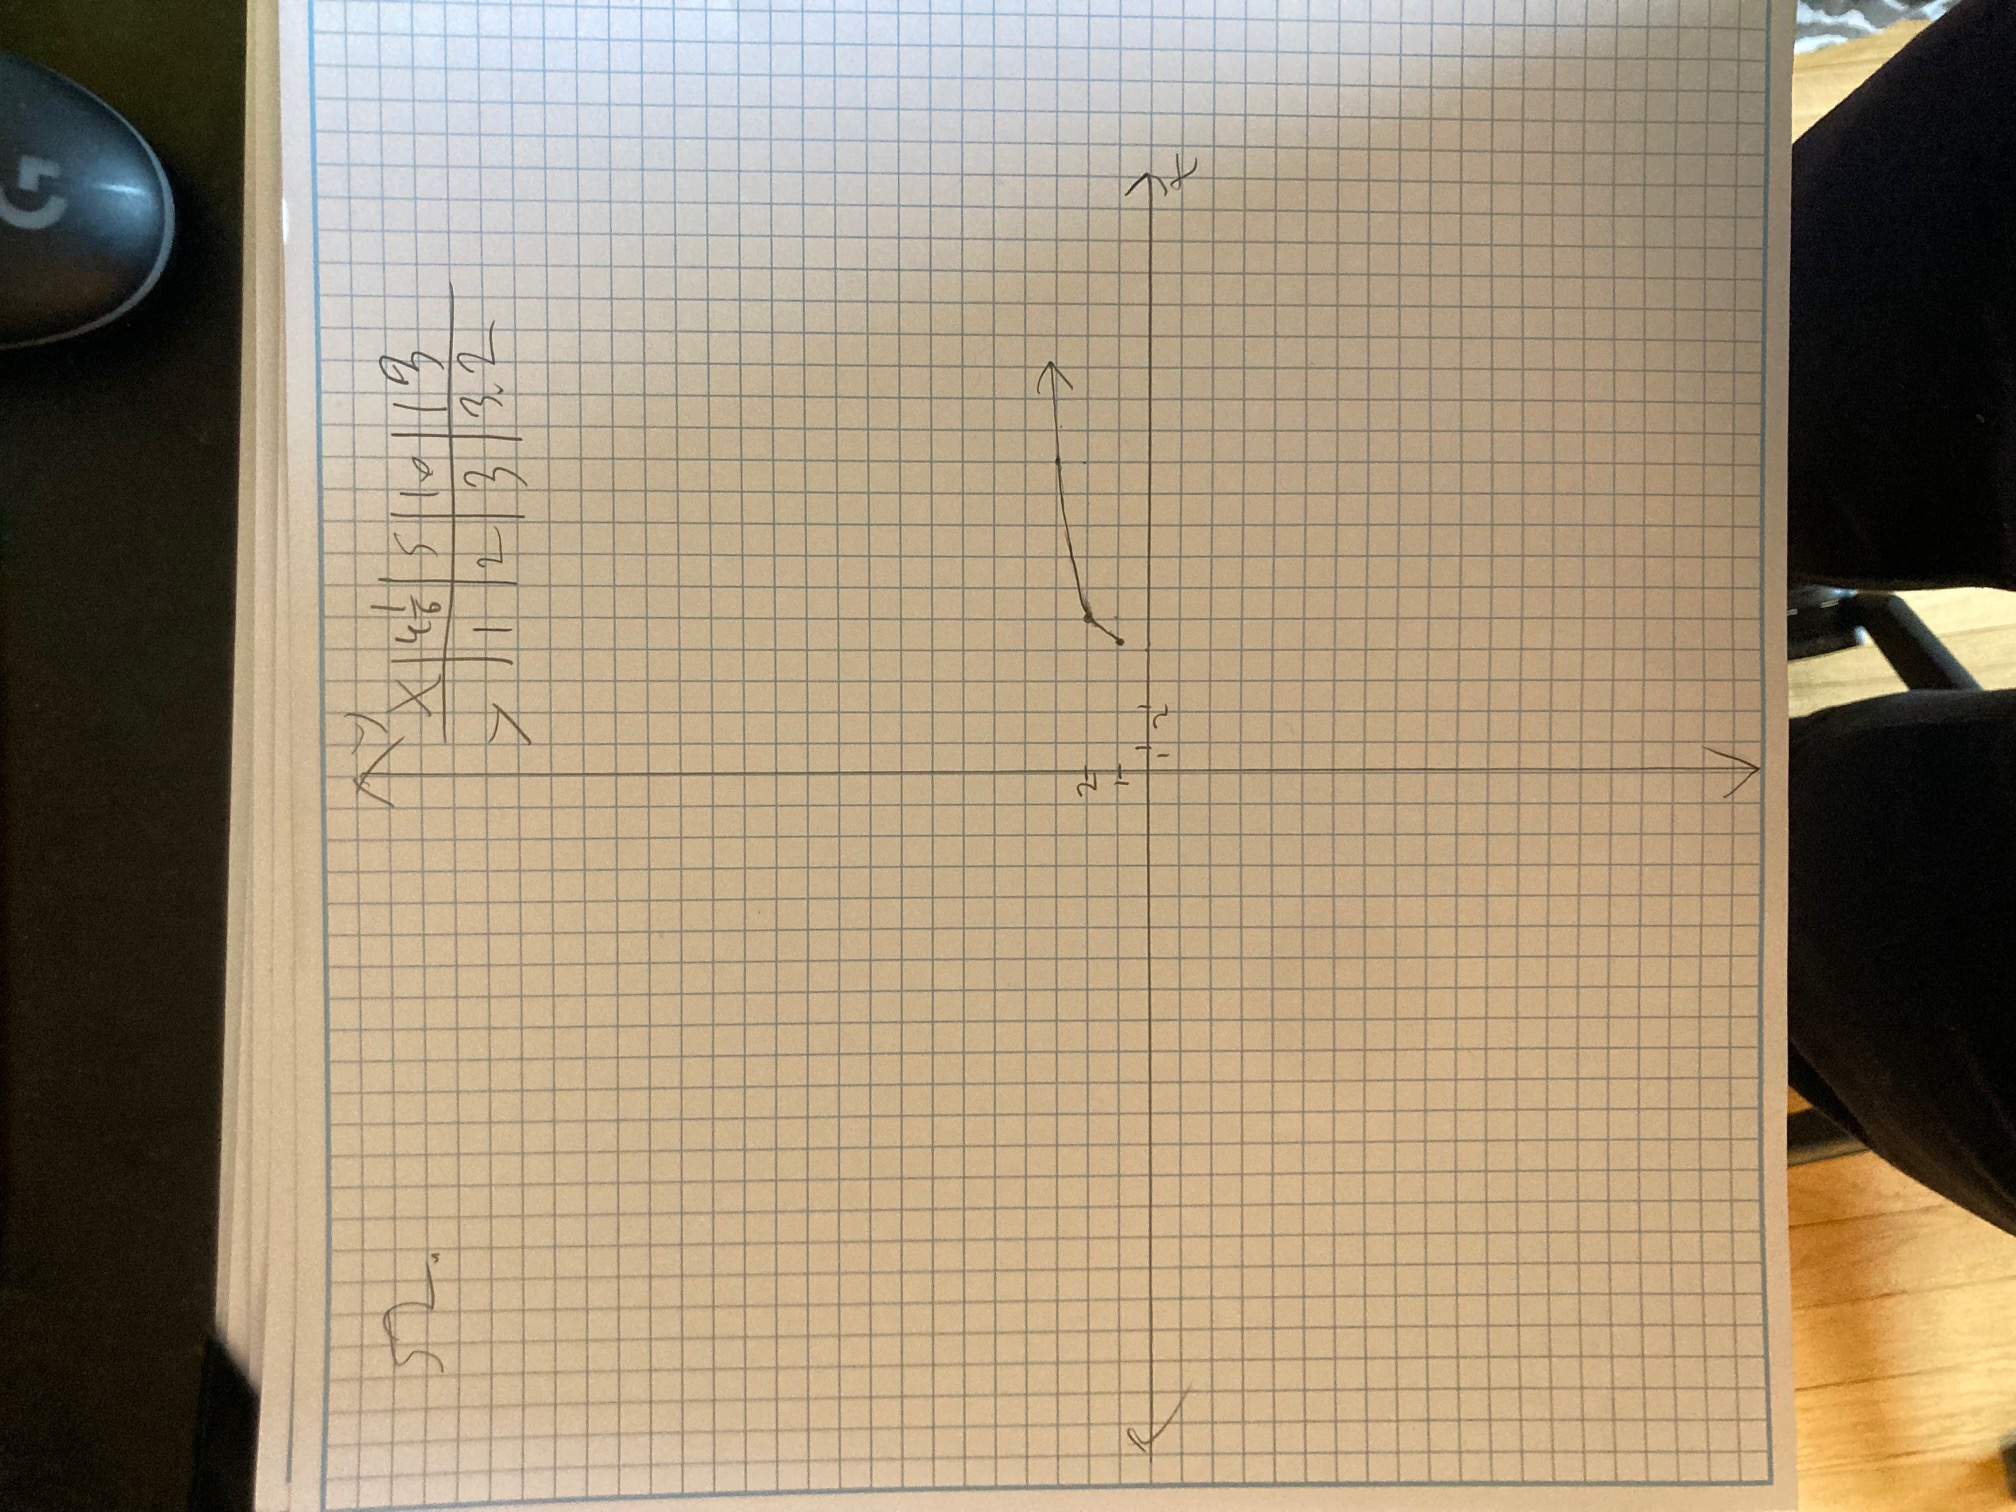
\includegraphics[width = 4in, height = 4in, angle=-90]{52}
\newline The domain of the function is $>4$, and the range of the function is all real numbers.

\section*{54}
\[ \log_{27}9=\log_{3^3}3^2=\frac{2}{3} \]

\section*{55}
\[ \log_{8}32=\log_{2^3}2^5=\frac{5}{3} \]

\section*{56}
\[ \log_{125}625=\log_{5^3}5^4=\frac{4}{3} \]

\section*{57}
\[ \log_4{128}=\log_{2^2}2^7=\frac{7}{2} \]

\section*{61}
(a): We are given that the release was $2.5\times 10^{24}$ ergs, meaning:
\[ M=0.29(\ln{2.5\times 10^{24}})-9.9\approx 0.29(56.12)-9.9\approx 6.37 \]


(b): We find the inverse of the model: \[ M=0.29(\ln{E})-9.9 \] \[ \frac{100M+990}{29}=\ln{E} \] \[ e^{\dfrac{100M+990}{29}}=E \] 
The above inverse functions represents the amount of energy $E$ released from an earthquake given an energy magnitude $M$.

\section*{63}
\[ s=0.159+0.118(\log{d}) \] \[ s-0.159=0.118(\log{d}) \] \[ \frac{1000s-159}{118}=\log{d} \] \[ 10^{\dfrac{1000s-159}{118}}=d \]
Suppose that $s=0.2$, meaning:
\[ 10^{\frac{1000(0.2)-159}{118}}=d \] \[ 10^{\frac{41}{118}}=d \] \[ d\approx 2.23 \]  milimeters.


\end{document} 
